%%==================================================
%% chapter02.tex for BIT Master Thesis
%% modified by 朱杰
%%==================================================
\chapter{研究基础}
本章作为全文研究的基础,主要将会对社交网络以及社区发现的相关概念进行阐述。首先将给出社交网络在维基百科中的定义,并对社交网络这一概念进行简单的描述;然后对社交网络的几大重要的统计特性进行了简要说明,包括节点的度、网络密度、平均路径长度、聚类系数和介数;接着将会阐述社交网络“小世界效应”和“无标度特性”这两个典型特征。在介绍完社交网络的相关概念之后,将直接引出本文的研究重点社区发现的相关概念。在给出了社区定义的前提之下,对社区发现这一概念进行了概要说明。

\section{社交网络}
\subsection{社交网络概述}
在维基百科中,社交网络(Social Network)被定义为“由许多节点以及节点间关系构成的一个网络结构。节点通常是指个人或组织(又称社团),社交网络代表各种社会关系”\cite{wiki:SN}。对社交网络的分析在早期只是针对现实生活中方便调查的关系进行分析。在国外曾有学者在研究如何减少政府机构的冗余行政人员以提高办事效率和降低政府开销时,就使用到了社交网络分析这一手段。通过私下采访和调查的手段,他们获取了某一政府机关几乎全部工作人员之间的来往接触关系,建立了一张交际网络。在对这张交际网络的分析时,他们发现其中有些节点在业务流程线上是属于多余的,其功能只是交接两边的节点。对于提高效率而言,分析此网络并减少这样无谓的节点即可有效的降低开销。不像早期的社交网络主要是通过合作关系建立起来的职业网络,如今随着互联网社交媒体的诞生和飞速发展,社交网络逐渐线上化。

本文所指的社交网络特指在线社交网络(下文统称社交网络)。现在人们所说的社交网络一般而言其实就指代在线社交软件,也就是在互联网上与其他人产生联系的一个平台。在线社交媒介主要有即时通讯类软件(例如微信、QQ)、在线社交类软件(例如Facebook、人人网)、微博类软件(例如新浪微博、Twitter)、贴吧类软件(例如百度贴吧、悟空问答、知乎)、博客分享类软件(例如CSDN、简书)、职场关系类软件(例如领英、脉脉)和短视频分享类软件(例如抖音、快手)等等。而社交网络就是在这些社交媒介中抽象虚拟出来的一张网络图,在这张图中,每个个人(或者组织)抽象为一个节点,而人与人之间(或者组织之间)的关系(或者互动)则抽象为边。每个账号在社交媒体上填写的基本信息就是其节点属性,同样节点彼此之间的边上也有着相应的边的属性。这一切就构成了一个社交网络结构。社交网络虽然是抽象出来的产物,但是其中的社会关系却都是真实的。图\ref{fig:fig2-1}展示了一个简单的社交网络抽象图。

\begin{figure}
  \centering
  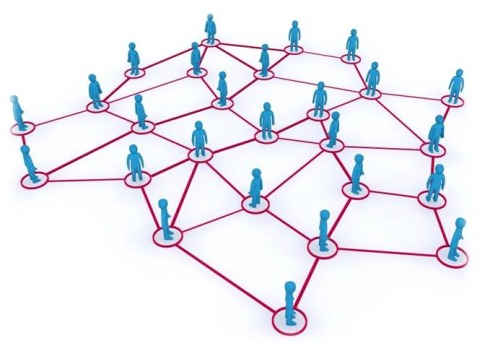
\includegraphics[width=0.75\textwidth]{figures/fig2-1}
  \caption{一个简单的社交网络抽象图}\label{fig:fig2-1}
\end{figure}

\subsection{社交网络的统计特性}
因为社交网络的本质其实就是一个由节点(人或组织)和边(社会关系)组成的图结构,所以社交网络模型之中的很多概念都来源于图论。在这一小节中,将会简单介绍社交网络中常用的几种统计概念,包括节点的度、网络密度、平均路径长度、边的介数和聚类系数。这些统计概念或多或少都旨在反映社交网络的一些特性,比如疏密程度、信息传播开销等等。

(1)节点的度(Degree)

在无向图中,任意节点的度即是与其相连的边的数目。而在有向图中,又可以细分为入度和出度,即分别以节点为终点和起点的边的数目。在社交网络之中,一个节点的度越大,就表示其在这个网络中扮演着越重要的角色。影响力越大的人,在网络中节点的度就越大。例如在微博上,明星拥有着众多的粉丝,而普通用户往往只有很少的粉丝,前者在社交网络中抽象成的节点的度就会很大,后者的度就会很小。网络的平均节点度就是网络中所有节点的度的平均值,它可以反映网络的疏密程度。此外,还可以通过节点度的分布来刻画描述不同节点的重要性。

(2)网络密度(Density)

在社交网络之中,网络密度被定义为网络中实际存在的边数与最多可容纳边数的比值。通常被用来测量社交网络中社交关系的紧密程度及其演变趋势,其计算方式可参考公式\ref{eqn:density}。如果一个社交网络的网络密度还很小,则说明该网络还尚且处在起步阶段;而若一个社交网络的网络密度已经比较大了,那么说明该网络已经比较成熟,网络之中几乎所有节点之间都有联系。

\begin{equation}
  \label{eqn:density}
  Density=\frac{2m}{n(n-1))} 
\end{equation}

公式\ref{eqn:density}中的n和m分别为社交网络中节点的数目和边的数目,且$Density\in [0,1]$。其中,当整个网络中没有一条边,即所有节点都独立存在时,$Density$取0;而当网络中所有节点之间都有边相连时,即网络处于全连接状态时,$Density$取1。一般而言,大规模的社交网络的密度会比中小规模的小一些,因此,不同规模社交网络之间的网络密度也就不具有可比性了。例如,分别以学校和家庭为规模建立一个社交关系网络,显然一个家庭关系的网络密度会大很多。

(3)平均路径长度(Average Path Length)

一个社交网络的平均路径长度被定义为:所有联通节点之间最短路径的平均值。即所有节点之间的最短路径上存在的节点个数的平均值。其计算方法可参考公式\ref{eqn:APL}。

\begin{equation}
  \label{eqn:APL}
  APL=\frac{2}{n(n-1)}\sum _{i=1}^{n}\sum_{j=1}^{n}d_{ij}
\end{equation}

公式\ref{eqn:APL}中的n为当前网络中节点的数目,$d_{ij}$为网络中节点$v_i$和$v_j$之间的最短路径。平均路径长度$APL$通常也是用于反映网络间的紧密程度的,一般也可叫做网络的平均距离。如果社交网络的平均路径长度比较大,则代表网络比较稀疏,节点之间进行信息传播的开销比较大;相反,若社交网络的平均路径长度小,则代表网络稠密,节点之间可以比较迅速快捷的进行消息传递。

(4)聚类系数(Clustering Coefficient)

根据图论,聚类系数表示的是一个图中节点汇聚程度的系数。在很多社交网络中,若节点$v_i$与节点$v_j$相连接,而节点$v_j$与节点$v_k$相连接,那么很大概率上节点$v_i$和节点$v_k$也会相连。这种现象也表明了社交网络中部分节点之间存在着密集连接的这一特性。在无向图中,节点$v_j$的聚类系数$CC_{v_j}$的计算方式可参考公式\ref{eqn:CC}。

\begin{equation}
  \label{eqn:CC}
  CC_{v_j}=\frac{n}{C_k^2}=\frac{2n}{k(k-1)}
\end{equation}

公式\ref{eqn:CC}中$k$表示节点$v_j$所拥有的邻居节点的数目,n表示节点$v_j$的所有相邻节点之间互相连接的边的数目。简而言之,聚类系数可以用来描绘社交网络中一个用户的朋友们之间也是朋友的概率,反映的也就是社交网络的聚集性。具体的,它还可以分为全局聚类系数和局部聚类系数,此处不再赘述。

(5)介数(Betweeness)

介数可以分为节点介数和边介数,表示的是网络图中某一节点或者某一条边被整个图中所有节点间的最短路径经过的概率之和。通常被用来评价节点的重要程度。在连接不同社区之间的中间节点(或者边)的介数就会比其他节点(或者边)的介数要大很多,这也反映了这类节点在社交平台中作为消息传播的核心地位及其重要程度。对于网络中任意节点v,其介数的计算方式可参考公式\ref{eqn:bet}。

\begin{equation}
  \label{eqn:bet}
  C_B(v)=\sum _{s\neq v\neq t \in V}\frac{\sigma_{st}(v)}{\sigma_{st}}
\end{equation}

在公式\ref{eqn:bet}中,$\sigma_{st}(v)$表示经过节点$v$的$s\rightarrow t$的最短路径条数,$\sigma_{st}$表示$s\rightarrow t$的最短路径条数。直观上来看,节点$v$的介数$C_B(v)$反映的是节点$v$作为“桥梁”或者“枢纽”的重要程度。

\subsection{社交网络的典型特征}
在社交网络之中普遍存在着两个典型的特征:小世界效应和无标度特性。

(1)小世界效应

1929年匈牙利作家F.Karinthy率先提出了“小世界现象(Small-world Effect)”的论断。他认为,平均来说地球上的任何两个人都可以通过一条由5位联系人组成的链条而联系起来。在1967年,美国哈佛大学的社会心理学教授Stanley Milgram提出了著名的“六度分隔(Six Degrees of Separation)假说”\cite{Milgram1967The},大意同样为任何两个想要取得联系的陌生人之间最多只隔着5个人,便可完成两人之间的联系。他通过设计了一个信件实验来证明他的猜想,实验大致经过为:他随机选择了300余人,每人分发一封信并指定各不相同的收信者;要求如果寄信者认识收信者,则直接寄出,否则就寄给一个自己认识的并且可能认识收信者的人,直至收信者收到信为止;实验最终共有约60人收到了信,而这些信平均经手了6次就到达了收信人手中。在1998年的时候,Duncan Watts和Steven Strogatz正式提出了小世界网络的概念并建立了小世界模型\cite{Watts1998Collectivedynamics}。文献中将小世界效应定义为:若网络中任意两个节点之间的平均距离(即平均路径长度APL)随网络中节点数n的增加呈对数增长,即$APL\sim ln(n)$,且网络的局部结构上仍然具有较明显的集团化特征。

小世界效应反映的是社交网络中任何用户之间都近在咫尺的现象,即:社交网络的平均路径长度都很短。小世界现象在在线社交网络中得到了很好地验证,根据2011年Facebook数据分析小组的报告,Facebook约7.2亿用户中任意两个用户间的平均路径长度仅为4.74,而这一指标在Twitter中为4.67。因此可以说,在五步之内,任何两个网络上的个体都可以互相连接。

(2)无标度特性

大多数社交网络都存在着少数节点的度极大,而大部分节点都只有较小的度这一现象。网络因为缺乏一个统一的衡量尺度而呈现出异质性,这种节点度分布不存在有限衡量分布范围的性质就被称为无标度。这其实体现的是社交网络中用户的度呈现出幂律分布(Power-law Distribution)的规律。幂律分布广泛存在于各个领域,其核心就是绝大部分事件的规模其实很小,但是极少数事件的规模却表现的相当大。例如:世界上绝大部分的财富都被掌握在极少数的超级富豪的手中;以网站的访问量而言,尽管互联网上为广大网民提供了无数的网页,但是大家每天访问量最多的仅仅就是几个熟悉的网页;在微博上,一个明星的粉丝可能有上百万乃至上千万,但是大部分普通人也只有寥寥无几的粉丝关注量。在直观上,这个现象就像图\ref{fig:fig2-2}中幂函数曲线一样。幂律分布其实体现的是一种极端的不平衡性。

\begin{figure}
  \centering
  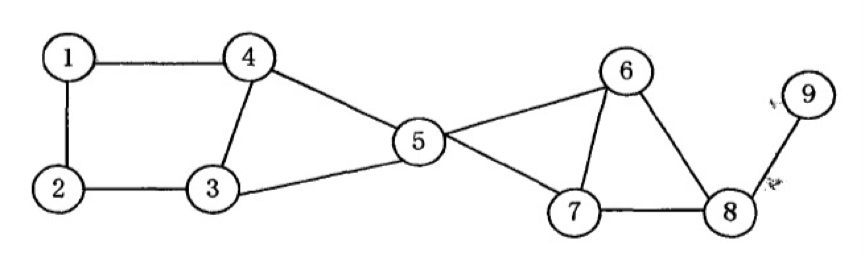
\includegraphics[width=0.75\textwidth]{figures/fig2-2}
  \caption{社交网络中度的幂律分布曲线}\label{fig:fig2-2}
\end{figure}

\section{社区发现}
\subsection{社区的定义}
社交网络除了小世界效应和无标度特性这两个典型特征之外,还有一个重要的一个特点就是“社区(Community)”的存在。也有部分学者将之译为“社团”,本文将之称为社区。在直观上,同现实生活中所说的社区一样,社交网络乃至复杂网络中的社区也可以简单地被理解为是一些彼此之间联系紧密的节点的集合,或者说是一些拥有共同或相似属性的个体组成的团体,这些集合或者团体对于分析社交网络有着至关重要的意义。目前在学术界对社区的概念尚且还没有一个完整统一的定义。本文下面从不同的角度给出了三种定义:基于网络拓扑结构的定义、基于节点相似度的定义和重叠社区的定义。

(1)基于网络拓扑结构的社区定义

将社交网络抽象成一个由节点(人或组织)和边(社会关系)组成的网络拓扑结构,那么一个社区即是指由若干个节点组成的具有高内聚特性的子集合。在这个子集合之中的节点彼此之间联系紧密,表现上就是子集内部节点之间存在着相对比较多的边;而在多个子集合之间,也就是社区之间联系比较稀疏,表现上就是存在着相对较少的边。图\ref{fig:fig2-3}所示即是一个具有社区结构的网络。图中的14个节点组成的网络拓扑图中形成了3个社区结构,为了更直观显示,三个社区的节点分别以黄色、蓝色和绿色三种颜色区分。此种定义对应的社区发现算法即是本文绪论第二小节国内外研究现状中提到的基于链接的社区发现算法。

\begin{figure}
  \centering
  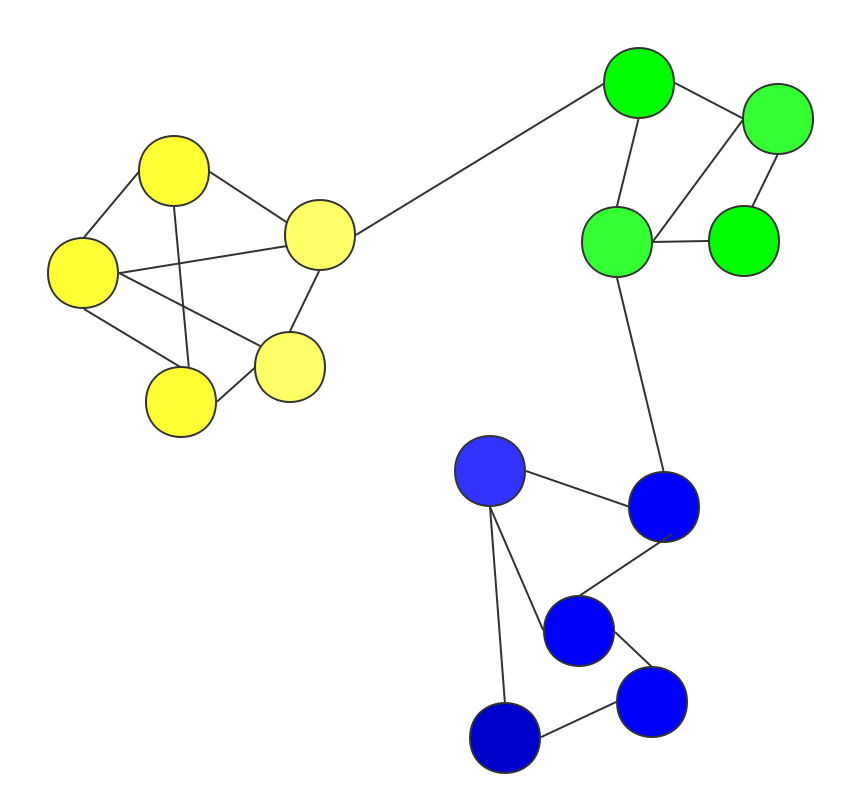
\includegraphics[width=0.75\textwidth]{figures/fig2-3}
  \caption{一个具有社区结构的网络示意图}\label{fig:fig2-3}
\end{figure}

(2)基于节点相似度的社区定义

这里定义的社区依然是由若干节点组成的子集合,但是在表现形式以及定量分析手段方面与上一种定义有所区别。基于节点相似度的社区定义认为属于同一个社区的节点都是相似的,而社区与社区之间的节点的相似度则较低。节点之间的相似度的高低依靠建立节点相似度模型来衡量。该定义相较基于网络拓扑结构的定义会更易于理解,因为社区本就是代表着社交网络中具有相同或者类似属性的元素的子集。此种定义对应的社区发现算法即是本文绪论第二小节国内外研究现状中提到的基于内容的社区发现算法。

其实在本质上,基于网络拓扑结构的社区定义和基于节点相似度的社区定义是一致的。两者都是将社区定义为网络中所有元素组成的集合的若干子集,在子集之中的元素基于某种因素会彼此连接紧密,而与其他子集内的元素连接稀疏。只不过两者对于元素之间的紧密与稀疏的定量分析手段不同,前者是根据网络的拓扑结构和节点之间的边的联系,而后者是根据节点的属性分析节点间相似度。

(3)重叠社区的定义

此前关于社区的定义都忽视了个体可能属于两个或更多社区的可能性。但是,许多真实的社交网络都存在着社区的重叠。例如,一个人可以同时属于家庭群体和朋友群体这两个社交群体。图\ref{fig:fig2-4}所示即是一个具有重叠社区结构的网络。图中的16个节点组成的网络拓扑图中形成了3个社区结构,三个社区的节点分别以黄色、蓝色和绿色三种颜色区分,而这其中有两个黄蓝相间的节点即是同时属于黄色代表的社区和蓝色代表的社区。重叠社区(Overlapping Community)和普通社区相比,唯一的差别就在于:代表重叠社区的子集之间可以有交集,而代表普通社区的子集之间是没有交集的。在包含重叠社区的网络中,这些重叠社区间的交集,即这些属于多个社区的元素(个体),对社区的演化和社区间的沟通都起到了极其重要的作用,因为它们就是不同社区之间的桥梁和纽带。一般而言,重叠社区结构也可以分为两种。一种是离散型重叠社区,即对于一个社区,某个节点只有属于和不属于这两个选择项。另一种是模糊型重叠社区,即每个节点有着对于不同社区的隶属度。关于重叠社区定义对应的社区发现算法即是本文绪论第二小节国内外研究现状中提到的重叠社区发现算法。

\begin{figure}
  \centering
  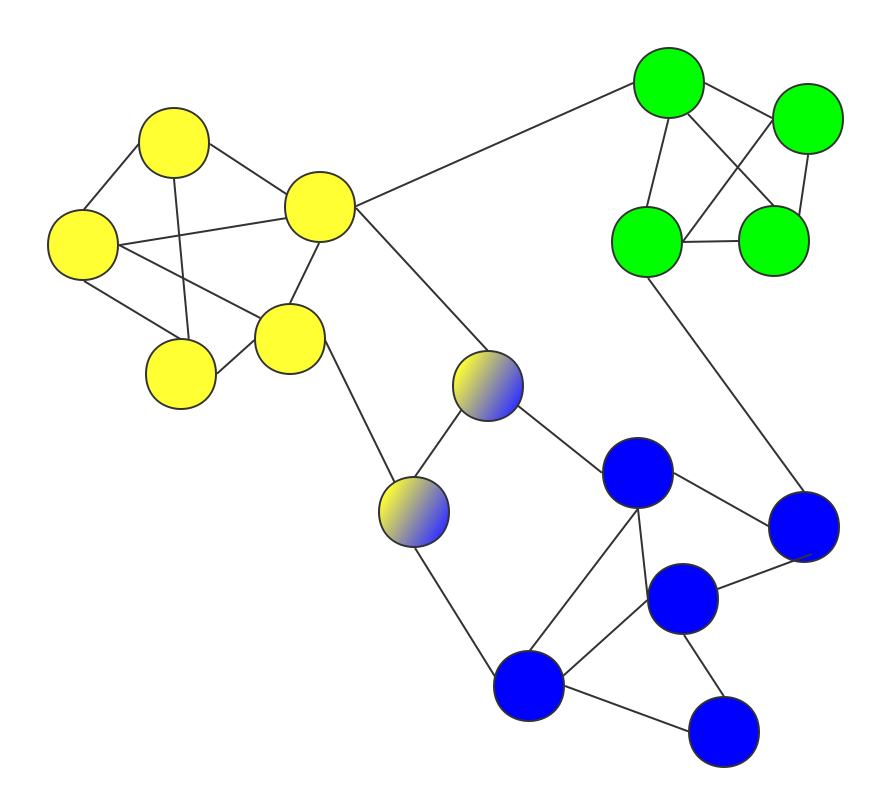
\includegraphics[width=0.75\textwidth]{figures/fig2-4}
  \caption{一个具有重叠社区的网络示意图}\label{fig:fig2-4}
\end{figure}

\subsection{社区发现概述}
上一小节已经较为详细的解释了社区的含义。那么给定一个网络图$G=(V,E)$,其中顶点集为$V$,边集为$E$,社区发现(Community Detection,也可以译作社区检测或者社团检测)即是在网络之中发现社区结构的过程。挖掘社交网络中的社区在人物分析、商业个性化推荐和舆情控制等领域均有着很关键的作用。

在社交网络之中,社区结构是客观存在的,但是往往人们只会与他们有直接接触的用户进行互动,而在同一个社区中,还存在着不少与他有着共性的用户,很可能他们有着共同的朋友但彼此之间却不了解,因此如果要进行朋友推荐,那么隶属于同一社区的成员之间就应该率先进行彼此推荐。此外,对一个大型网络调用社区发现算法,其实是对其按照某种标准进行了划分,在此基础上可对每个社区做进一步的发掘。而从计算的角度而言,社区划分相当于分解了任务,起到了降低计算复杂度的作用。并且目前的社交软件上用户广泛,无法将所有用户的信息都存储在同一台服务器之上,这就必须要使用到分布式存储。在分布式存储中,如果不经过分类杂乱无章的进行存储,那么最终将导致巨大的通信开销,而如若先将社交网络进行社区发现,把同一社区内的用户存储在同一服务器内,这就可以省下大笔的通信开销,大大提高社交平台的性能。

近年来,对社交网络中的社区结构进行检测并分析已经吸引了众多研究人员的关注,一大批社区发现算法也随之被提出。在本文绪论第二小节国内外研究现状中将社区发现算法分为了基于链接的算法、基于内容的算法和融合了链接与内容的算法。对于社区的重叠问题,还可以将社区发现分为非重叠和重叠的社区发现,在本文的国内外研究现状中也有对重叠社区发现算法进行了简单的综述。因此,对于具体的社区发现算法,此处不再赘述。

\section{本章小结}
本章主要是对社交网络以及社区发现的相关概念进行了综述。首先给出了社交网络在维基百科中的定义,在此基础上对社交网络这一概念进行了简单的描述;其次对社交网络的五大重要的统计特性以及两大典型特征进行了一一说明;接着从三个不同角度对社区的定义进行了详细介绍,最后引出了社区发现这一概念,并对其进行了必要的介绍。



